\documentclass[11pt,a4paper]{article}
\usepackage[utf8]{inputenc}
\usepackage[margin=0.85in]{geometry}
\usepackage{amsmath,amssymb,amsthm}
\usepackage{xcolor}
\usepackage{tcolorbox}
\usepackage{tikz}
\usetikzlibrary{shapes,arrows,positioning,calc,decorations.pathreplacing}
\usepackage{booktabs}
\usepackage{array}
\usepackage{fancyhdr}
\usepackage{hyperref}
\usepackage{microtype}

% Color Palette Definitions
\definecolor{primarynavy}{RGB}{26, 54, 93}       % #1A365D - Deep Navy
\definecolor{secondaryteal}{RGB}{13, 148, 136}   % #0D9488 - Teal Accent
\definecolor{darkslate}{RGB}{45, 55, 72}        % #2D3748 - Body Text
\definecolor{lightbg}{RGB}{247, 250, 252}        % #F7FAFC - Soft Background
\definecolor{accentblue}{RGB}{49, 130, 206}      % #3182CE - Bright Blue
\definecolor{warmgold}{RGB}{214, 158, 46}        % #D69E2E - Gold Highlight

\hypersetup{
    colorlinks=true,
    linkcolor=primarynavy,
    citecolor=secondaryteal,
    urlcolor=accentblue,
    pdftitle={Lecture Notes: Analytic Geometry (Polar Coordinates \& Conics)},
    pdfauthor={Class Notes}
}

% Page Setup
\pagestyle{fancy}
\fancyhf{}
\fancyhead[L]{\small \textbf{\color{primarynavy}Analytic Geometry}}
\fancyhead[R]{\small \textbf{\color{secondaryteal}MATMJ52}}
\fancyfoot[L]{\small \textcolor{primarynavy}{\href{https://www.sciqb.com}{\textbf{www.sciqb.com}}}}
\fancyfoot[C]{\thepage}
\fancyfoot[R]{\small \textcolor{secondaryteal}{\href{https://www.sciqb.com}{\textbf{SCIQB Platform}}}}
\renewcommand{\headrulewidth}{0.6pt}
\renewcommand{\footrulewidth}{0.4pt}

% Custom TColorBox Environments
\newtcolorbox{defbox}[1]{
    colback=lightbg,
    colframe=primarynavy,
    fonttitle=\bfseries\color{white},
    title={#1},
    boxrule=1pt,
    top=3mm, bottom=3mm, left=4mm, right=4mm
}

\newtcolorbox{formulabox}[1]{
    colback=secondaryteal!8!white,
    colframe=secondaryteal,
    fonttitle=\bfseries\color{white},
    title={#1},
    boxrule=1pt,
    top=3mm, bottom=3mm, left=4mm, right=4mm
}

\newtcolorbox{exbox}[1]{
    colback=white,
    colframe=accentblue,
    fonttitle=\bfseries\color{white},
    title={#1},
    boxrule=1pt,
    top=3mm, bottom=3mm, left=4mm, right=4mm
}

\setlength{\parindent}{0pt}
\setlength{\parskip}{6pt}

\begin{document}

% Title Banner
\begin{center}
    \tcbset{colframe=primarynavy,colback=primarynavy!5!white,arc=0mm}
    \begin{tcolorbox}[sharp corners, boxrule=1.5pt]
        \begin{center}
            {\Large \bfseries \color{primarynavy} ANALYTIC GEOMETRY}\\[4pt]
            {\large \bfseries \color{secondaryteal} Polar Coordinates, Distance Formula, Area of Triangle \& Conic Sections}\\[6pt]
            {\small \textbf{Course Code:} MATMJ52 \quad|\quad \textbf{Platform:} \href{https://www.sciqb.com}{\color{accentblue}\textbf{www.sciqb.com}}}
        \end{center}
    \end{tcolorbox}
\end{center}

\vspace{0.3cm}

\section{Introduction to Polar Coordinates}

In two-dimensional geometry, a point in a plane can be uniquely represented using a distance and an angle relative to a fixed reference point and direction. This system is known as the \textbf{Polar Coordinate System}.

\begin{defbox}{Definitions: Components of Polar Coordinates}
\begin{itemize}
    \item \textbf{Pole (or Origin) [$O$]:} A fixed reference point in the plane, denoted by $O$.
    \item \textbf{Initial Line [$OX$]:} A fixed horizontal straight line emanating from the pole $O$ extending to the right.
    \item \textbf{Radius Vector [$r$]:} The line segment $OP$ connecting the pole $O$ to any point $P$ in the plane. Its length is denoted by $r = |OP| \ge 0$.
    \item \textbf{Vectorial Angle [$\theta$]:} The angle measured counter-clockwise from the initial line $OX$ to the radius vector $OP$. It is denoted by $\theta = \angle XOP$.
\end{itemize}
Thus, any point $P$ is represented by the ordered pair $(r, \theta)$.
\end{defbox}

\subsection{Transformation between Cartesian and Polar Coordinates}

Let $P(x, y)$ be a point in the Cartesian coordinate system with the origin coinciding with the pole $O$ and the positive $x$-axis coinciding with the initial line $OX$. Drop a perpendicular $PN$ from $P$ onto $OX$.

\begin{center}
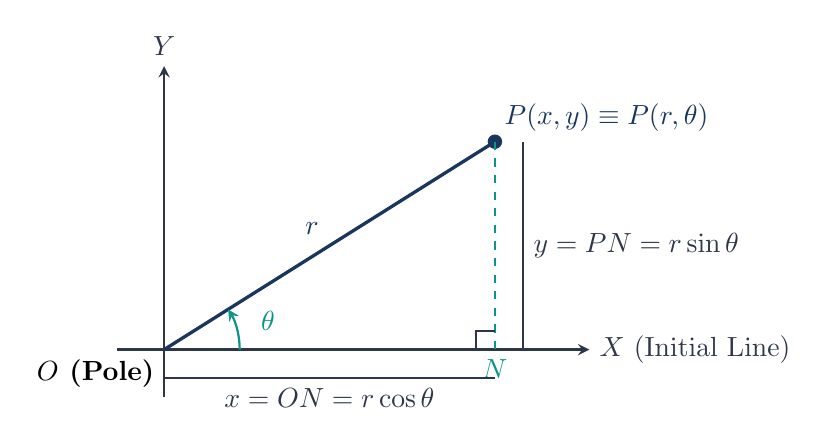
\begin{tikzpicture}[scale=1.2, >=stealth]
    % Axes
    \draw[->, thick, color=darkslate] (-0.5,0) -- (4.5,0) node[right] {$X$ (Initial Line)};
    \draw[->, thick, color=darkslate] (0,-0.5) -- (0,3) node[above] {$Y$};
    
    % Origin
    \node[below left, font=\bfseries] at (0,0) {$O$ (Pole)};
    
    % Point P
    \coordinate (P) at (3.5, 2.2);
    \filldraw[color=primarynavy] (P) circle (2pt) node[above right, font=\bfseries] {$P(x,y) \equiv P(r,\theta)$};
    
    % Radius vector r
    \draw[line width=1.2pt, color=primarynavy] (0,0) -- (P) node[midway, above left, font=\bfseries] {$r$};
    
    % Perpendicular PN
    \draw[dashed, thick, color=secondaryteal] (3.5, 2.2) -- (3.5, 0) node[below, font=\bfseries] {$N$};
    \draw[thick, color=darkslate] (3.3,0) -- (3.3,0.2) -- (3.5,0.2);
    
    % Lengths
    \draw[thick, color=darkslate] (0,-0.3) -- (3.5,-0.3) node[midway, below] {$x = ON = r \cos \theta$};
    \draw[thick, color=darkslate] (3.8,0) -- (3.8,2.2) node[midway, right] {$y = PN = r \sin \theta$};
    
    % Angle theta
    \draw[->, thick, color=secondaryteal] (0.8,0) arc (0:32.14:0.8);
    \node[color=secondaryteal, font=\bfseries] at (1.1, 0.3) {$\theta$};
\end{tikzpicture}
\end{center}

From the right-angled triangle $\triangle ONP$:
\begin{enumerate}
    \item \textbf{Cartesian in terms of Polar Coordinates:}
    \begin{equation}
        \label{eq:cartesian_from_polar}
        ON = x = r \cos \theta \quad \text{and} \quad PN = y = r \sin \theta
    \end{equation}

    \item \textbf{Polar in terms of Cartesian Coordinates:}
    Squaring and adding equations (\ref{eq:cartesian_from_polar}):
    \begin{equation}
        x^2 + y^2 = r^2 \cos^2 \theta + r^2 \sin^2 \theta = r^2 \implies r = \sqrt{x^2 + y^2}
    \end{equation}
    Dividing $y$ by $x$:
    \begin{equation}
        \tan \theta = \frac{PN}{ON} = \frac{y}{x} \implies \theta = \tan^{-1}\left(\frac{y}{x}\right)
    \end{equation}
\end{enumerate}

\section{Distance Between Two Points in Polar Coordinates}

Let $P(r_1, \theta_1)$ and $Q(r_2, \theta_2)$ be two given points in polar coordinates with respect to the pole $O$ and initial line $OX$.

\begin{center}
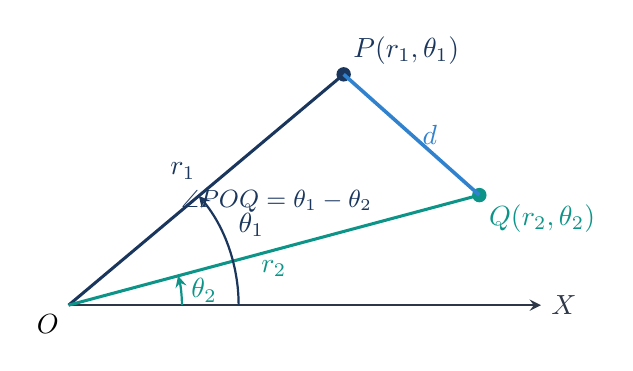
\begin{tikzpicture}[scale=1.2, >=stealth]
    % Initial line
    \draw[->, thick, color=darkslate] (0,0) -- (5,0) node[right] {$X$};
    \node[below left, font=\bfseries] at (0,0) {$O$};
    
    % Point P
    \coordinate (P) at (40:3.8);
    \filldraw[color=primarynavy] (P) circle (2pt) node[above right, font=\bfseries] {$P(r_1, \theta_1)$};
    \draw[line width=1.1pt, color=primarynavy] (0,0) -- (P) node[midway, above left] {$r_1$};
    
    % Point Q
    \coordinate (Q) at (15:4.5);
    \filldraw[color=secondaryteal] (Q) circle (2pt) node[below right, font=\bfseries] {$Q(r_2, \theta_2)$};
    \draw[line width=1.1pt, color=secondaryteal] (0,0) -- (Q) node[midway, below] {$r_2$};
    
    % Line PQ
    \draw[line width=1.3pt, color=accentblue] (P) -- (Q) node[midway, right, font=\bfseries] {$d$};
    
    % Angles
    \draw[->, thick, color=secondaryteal] (1.2,0) arc (0:15:1.2) node[midway, right] {$\theta_2$};
    \draw[->, thick, color=primarynavy] (1.8,0) arc (0:40:1.8) node[midway, above right] {$\theta_1$};
    
    % Angle POQ
    \node[color=primarynavy, font=\small] at (2.2, 1.1) {$\angle POQ = \theta_1 - \theta_2$};
\end{tikzpicture}
\end{center}

In $\triangle POQ$:
\begin{itemize}
    \item $OP = r_1$, \quad $OQ = r_2$
    \item $\angle POQ = |\theta_2 - \theta_1|$
\end{itemize}

By applying the \textbf{Law of Cosines} in $\triangle POQ$:
$$PQ^2 = OP^2 + OQ^2 - 2 \cdot OP \cdot OQ \cdot \cos(\angle POQ)$$
$$PQ^2 = r_1^2 + r_2^2 - 2 r_1 r_2 \cos(\theta_2 - \theta_1)$$

\begin{formulabox}{Polar Distance Formula}
The distance $d = PQ$ between two points $P(r_1, \theta_1)$ and $Q(r_2, \theta_2)$ is given by:
\begin{equation}
    PQ = \sqrt{r_1^2 + r_2^2 - 2 r_1 r_2 \cos(\theta_2 - \theta_1)}
\end{equation}
\end{formulabox}

\section{Area of a Triangle in Polar Coordinates}

Consider a triangle $\triangle ABC$ with vertices in polar coordinates given by $A(r_1, \theta_1)$, $B(r_2, \theta_2)$, and $C(r_3, \theta_3)$.

\begin{center}
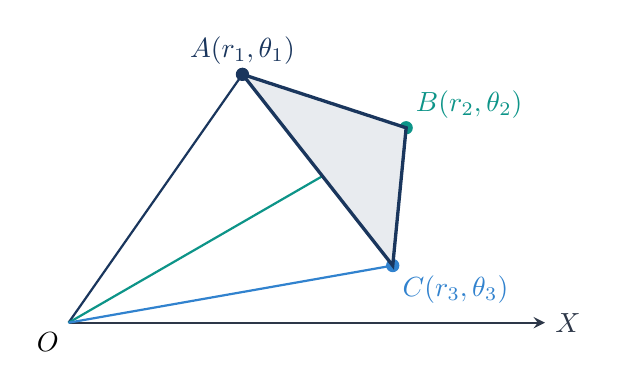
\begin{tikzpicture}[scale=1.1, >=stealth]
    \draw[->, thick, color=darkslate] (0,0) -- (5.5,0) node[right] {$X$};
    \node[below left, font=\bfseries] at (0,0) {$O$};
    
    \coordinate (A) at (55:3.5);
    \coordinate (B) at (30:4.5);
    \coordinate (C) at (10:3.8);
    
    \filldraw[color=primarynavy] (A) circle (2pt) node[above] {$A(r_1, \theta_1)$};
    \filldraw[color=secondaryteal] (B) circle (2pt) node[above right] {$B(r_2, \theta_2)$};
    \filldraw[color=accentblue] (C) circle (2pt) node[below right] {$C(r_3, \theta_3)$};
    
    \draw[thick, color=primarynavy] (0,0) -- (A);
    \draw[thick, color=secondaryteal] (0,0) -- (B);
    \draw[thick, color=accentblue] (0,0) -- (C);
    
    \draw[line width=1.2pt, color=primarynavy, fill=primarynavy!10] (A) -- (B) -- (C) -- cycle;
\end{tikzpicture}
\end{center}

The area of $\triangle ABC$ can be obtained by summing/subtracting the areas of triangles formed with the pole $O$:
$$\text{Area}(\triangle ABC) = \text{Area}(\triangle AOB) + \text{Area}(\triangle AOC) - \text{Area}(\triangle BOC)$$

Recall that the area of any triangle with sides $a, b$ and included angle $\alpha$ is $\frac{1}{2} a b \sin \alpha$. Therefore:
$$\text{Area}(\triangle AOB) = \frac{1}{2} r_1 r_2 \sin(\theta_2 - \theta_1)$$
$$\text{Area}(\triangle BOC) = \frac{1}{2} r_2 r_3 \sin(\theta_3 - \theta_2)$$
$$\text{Area}(\triangle AOC) = \frac{1}{2} r_1 r_3 \sin(\theta_3 - \theta_1) = -\frac{1}{2} r_1 r_3 \sin(\theta_1 - \theta_3)$$

Combining these yields the general area formula:

\begin{formulabox}{Area of Triangle in Polar Coordinates}
The area of triangle $\triangle ABC$ with vertices $A(r_1,\theta_1), B(r_2,\theta_2), C(r_3,\theta_3)$ is:
\begin{equation}
    \text{Area}(\triangle ABC) = \frac{1}{2} \Big| r_1 r_2 \sin(\theta_2 - \theta_1) + r_2 r_3 \sin(\theta_3 - \theta_2) + r_3 r_1 \sin(\theta_1 - \theta_3) \Big|
\end{equation}
\end{formulabox}

\section{Polar Equation of a Conic Section}

\begin{defbox}{Definition: Conic Section}
A \textbf{conic section} (or simply conic) is defined as the locus of a moving point $P$ in a plane such that the ratio of its distance from a fixed point $S$ (called the \textbf{focus}) to its perpendicular distance from a fixed straight line $MX$ (called the \textbf{directrix}) is always constant.

This constant ratio is called the \textbf{eccentricity} of the conic, denoted by $e$:
\begin{equation}
    \frac{SP}{PM} = e
\end{equation}
\end{defbox}

\begin{center}
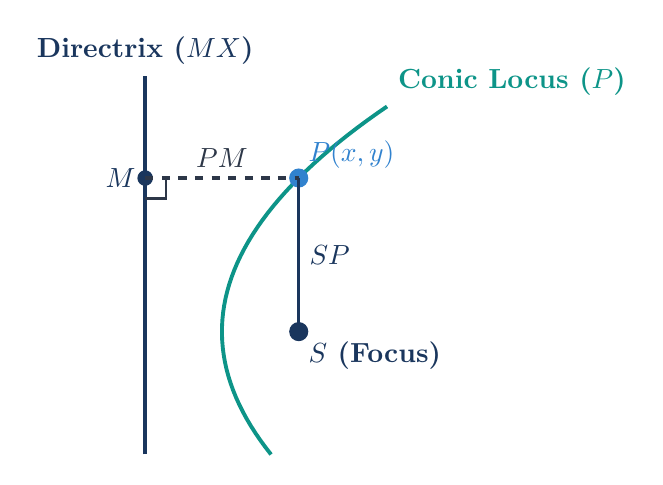
\begin{tikzpicture}[scale=1.3, >=stealth]
    % Directrix line
    \draw[line width=1.4pt, color=primarynavy] (0,-0.2) -- (0,3.5) node[above, font=\bfseries] {Directrix ($MX$)};
    
    % Point M on Directrix
    \coordinate (M) at (0, 2.5);
    \filldraw[color=primarynavy] (M) circle (2pt) node[left, font=\bfseries] {$M$};
    
    % Focus S
    \coordinate (S) at (1.5, 1.0);
    \filldraw[color=primarynavy] (S) circle (2.5pt) node[below right, font=\bfseries] {$S$ (Focus)};
    
    % Moving Point P on the curve (x = 1.5, y = 2.5)
    \coordinate (P) at (1.5, 2.5);
    
    % Smooth Mathematically Exact Parabola Locus: x = 0.75 + (y - 1)^2 / 3
    \draw[line width=1.4pt, color=secondaryteal, domain=-0.2:3.2, samples=50] 
        plot ({0.75 + (\x - 1.0)^2 / 3}, \x) node[above right, font=\bfseries] {Conic Locus ($P$)};
    
    % Point P mark
    \filldraw[color=accentblue] (P) circle (2.5pt) node[above right, font=\bfseries] {$P(x,y)$};
    
    % Distance SP (Line from S to P)
    \draw[line width=1.2pt, color=primarynavy] (S) -- (P) node[midway, right, font=\bfseries] {$SP$};
    
    % Perpendicular distance PM (Dashed line from M to P)
    \draw[line width=1.2pt, dashed, color=darkslate] (M) -- (P) node[midway, above, font=\bfseries] {$PM$};
    
    % Right angle symbol at M
    \draw[thick, color=darkslate] (0, 2.3) -- (0.2, 2.3) -- (0.2, 2.5);
\end{tikzpicture}
\end{center}

\subsection{Classification of Conics based on Eccentricity (\texorpdfstring{$e$}{e})}

Depending on the value of eccentricity $e$, the locus of point $P$ forms three fundamental conics:
\begin{enumerate}
    \item \textbf{Parabola ($e = 1$):} Here $SP = PM$. The locus is a parabola.
    \item \textbf{Ellipse ($e < 1$):} Here $SP < PM$. The locus is an ellipse.
    \item \textbf{Hyperbola ($e > 1$):} Here $SP > PM$. The locus is a hyperbola.
\end{enumerate}

\section{Theory of Pole and Polar}

\begin{defbox}{Definition: Pole and Polar}
If chords of a conic section are drawn through a fixed point $P$, and tangents are drawn at the extremities ($A$ and $B$) of all such chords, then the locus of the point of intersection of these two tangents is a straight line called the \textbf{Polar} of the fixed point $P$.

The fixed point $P$ itself is called the \textbf{Pole} of that straight line.
\end{defbox}

\begin{center}
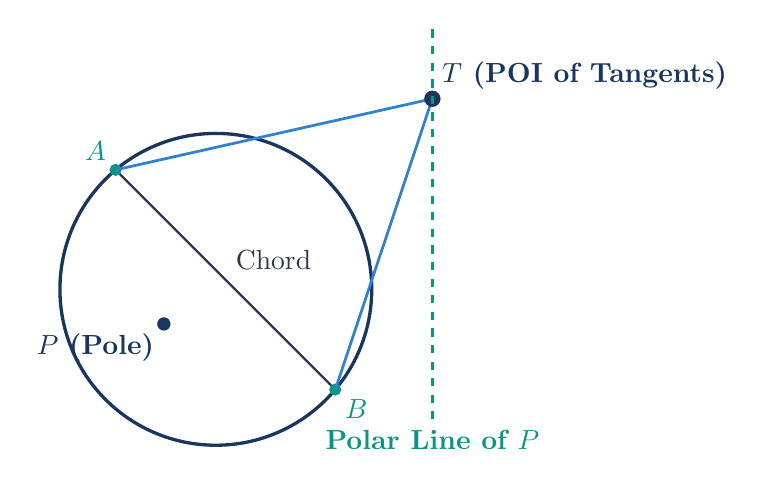
\begin{tikzpicture}[scale=1.1, >=stealth]
    % Circle / Conic
    \draw[line width=1.2pt, color=primarynavy] (0,0) circle (1.8cm);
    
    % Fixed point inside/outside
    \coordinate (P) at (-0.6, -0.4);
    \filldraw[color=primarynavy] (P) circle (2pt) node[below left, font=\bfseries] {$P$ (Pole)};
    
    % Chord AB through P
    \coordinate (A) at (130:1.8);
    \coordinate (B) at (-40:1.8);
    \draw[thick, color=darkslate] (A) -- (B) node[midway, above right] {Chord};
    \filldraw[color=secondaryteal] (A) circle (1.8pt) node[above left] {$A$};
    \filldraw[color=secondaryteal] (B) circle (1.8pt) node[below right] {$B$};
    
    % Tangents at A and B
    \draw[line width=1pt, color=accentblue] (A) -- (2.5, 2.2);
    \draw[line width=1pt, color=accentblue] (B) -- (2.5, 2.2);
    
    % Intersection point T
    \coordinate (T) at (2.5, 2.2);
    \filldraw[color=primarynavy] (T) circle (2.5pt) node[above right, font=\bfseries] {$T$ (POI of Tangents)};
    
    % Polar line
    \draw[line width=1.3pt, color=secondaryteal, dashed] (2.5, 3.0) -- (2.5, -1.5) node[below, font=\bfseries] {Polar Line of $P$};
\end{tikzpicture}
\end{center}

\section{Summary of Key Formulas}

\begin{formulabox}{Analytic Geometry Quick Reference Sheet}
\begin{enumerate}
    \item \textbf{Cartesian to Polar:} $x = r \cos \theta, \quad y = r \sin \theta$
    \item \textbf{Polar to Cartesian:} $r = \sqrt{x^2 + y^2}, \quad \theta = \tan^{-1}\left(\frac{y}{x}\right)$
    \item \textbf{Polar Distance Formula:} $d = \sqrt{r_1^2 + r_2^2 - 2 r_1 r_2 \cos(\theta_2 - \theta_1)}$
    \item \textbf{Area of Polar Triangle:} 
    $$\text{Area} = \frac{1}{2} \Big| r_1 r_2 \sin(\theta_2 - \theta_1) + r_2 r_3 \sin(\theta_3 - \theta_2) + r_3 r_1 \sin(\theta_1 - \theta_3) \Big|$$
    \item \textbf{Conic Eccentricity Ratio:} $\frac{SP}{PM} = e \quad \left(\text{Parabola: } e = 1, \quad \text{Ellipse: } e < 1, \quad \text{Hyperbola: } e > 1\right)$
\end{enumerate}
\end{formulabox}

\end{document}
